\subsection{Konstruktion der Mechanik}
Das Gestell des Edubot Modells wurde zum Großteil aus einfachen Dreischichtplatten gebaut. Vor dem Bau des Modells war eine ausgiebige Planungs- und Kontstruktionsphase erforderlich, in der auch ein ein Maßstabsgetreues 3D Modell des Roboters in Google Sketch up erstellt wurde.
Teilweise konnten vor allem für die Konstruktion von komplexeren Bauteilen wie den Gelenken Konzepte verwendet und angepasst werden, die bereits für die leistungsfähigere Mechanik des KEBA Modells entwickelt wurden.
Bei der Konstruktion und beim Erstellen des 3D Modells wurden wir tatkräftig von Herrn Konrad Maier unterstützt, da es uns hier schlichtweg an Erfahrung fehlte.
Im Hinblick auf eine mögliche Erweiterbarkeit des Edubot Modells durch verschiedene Werkzeuge oder eine weitere Achse wurde viel Wert auf eine hohe Belastbarkeit der Konstruktion gelegt.
Die Folgende Abbildung zeigt das in Google SketchUp gefertigte 3D Modell:

\begin{figure}[H]
  \centering
  \begin{minipage}[t]{12 cm}
  	\centering
  	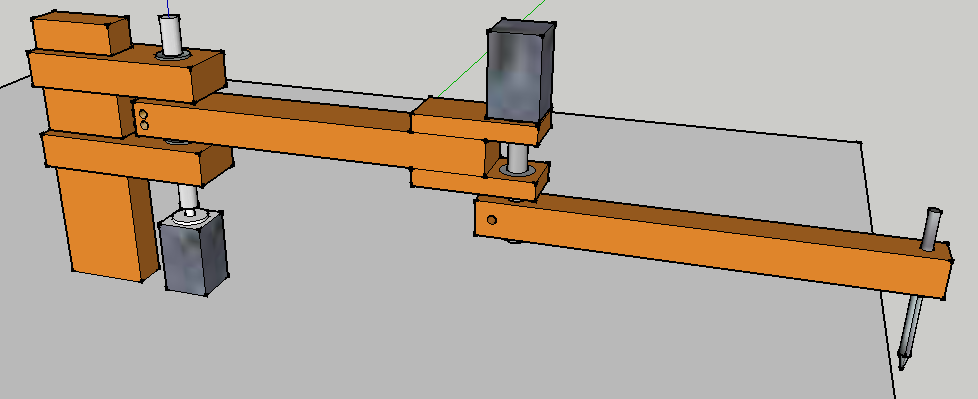
\includegraphics[width=12cm]{images/edubot_complete} 
    \caption{3D Modell der Konstruktion}
  \end{minipage}
\end{figure}

Besondere Herausforderungen stellten sich bei der Konstruktion des Holzmodells vor allem bei der Planung der Gelenke und beim finden einer Möglichkeit zum Verbinden der Motoren mit den Wellenverlängerungen:
\begin{itemize}
\item \textbf{Konzeption der Gelenke}\\
Bei der Planung der Gelenke musste eine Möglichkeit gefunden werden zu verhindern, dass das Gewicht der Achse in irgendeiner Weise direkt von der Motorachse getragen werden muss. Zusätzlich musste sichergestellt werden, dass die Achse möglichst leichtgängig ist um keine Leistung der ohnehin unterdimensionierten in Form von Reibungsverlust zu verschwenden.

Zur Erfüllung dieser Anforderungen war bereits bei der Grobplanung des KEBA Modells eine einfache, U-Förmige Konstruktion die mit Hilfe zweier Kugellager und einer Verlängerung der Motorwelle entwickelt worden. Diese geplante Konstruktion musst noch auf die Vorraussetzungen des Edubot-Modells angepasst werden. Die Folgende Abbildung zeigt am Beispiel der primären Achse, wie das beschriebene Problem gelöst wurde.

\begin{figure}[H]
  \centering
  \begin{minipage}[t]{8 cm}
  	\centering
  	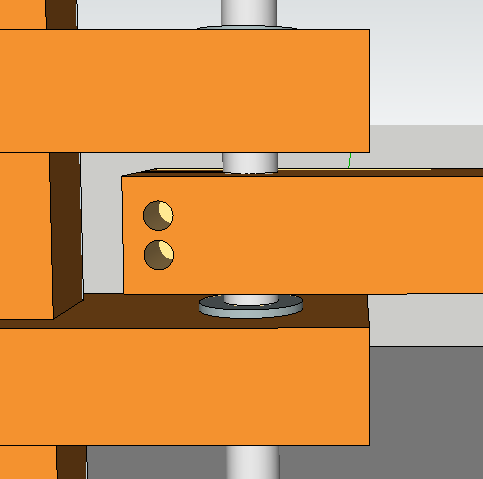
\includegraphics[width=8cm]{images/primary_gelenk} 
    \caption{Gelenk der primären Achse}
  \end{minipage}
\end{figure}

\item \textbf{Verbindung mit den Motoren}\\
Da die Motorwellen der vorhandenen Schrittmotoren weder über Zahnräder, noch etwaige Abflachungen oder Ähnliche Anschlussmöglichkeiten verfügen, stellte das Verbinden des Motors mit dem Modell eine unerwartet große Herausforderung dar. Da es mitunter beim Beschleunigen und Bremsen, verursacht durch die Wirkenden Hebelkräfte, zu einer nicht zu einer beträchtlichen Belastung dieser Kupplung kommen kann war die wichtigste Anforderung hierfür vor allem das Verhindern eines "Durchrutschen" des Motors. 

Gelöst wurde dieses Problem durch ein Stück Gummischlauch, welches exakt den Zwischenraum zwischen Motorwelle und der benötigten Wellenverängerung ausfüllte. Dieser Gummischlauch wurde über die Motorwelle gezogen, anschließend wurde die zuvor eingeschnittene Wellenverlängerung über die Motorwelle gestülpt. Im fall der primären Motorwelle wurde zur fixierung noch eine passende [todo] an der Verbindungsstelle angebracht um von außen Druck auszuüben und durch zusammenpressen von Motorwelle und Wellenverlängerung ein Durchrutschen zu verhindern. Im fall der sekundären Motorwelle wird das die selbe Aufgabe vom Kugellager erledigt. Abbildungen auf denen die beschriebene Problemlösung ersichtlich ist finden sich im Kapitel "'Bau der Mechanik".'
\end{itemize}